\section{Low-power Graphics Library}
\label{sec:system}

    
%%%%%%%%%%%%%%%%%%%%%%%%%%%%%%%%% 80 CHAR %%%%%%%%%%%%%%%%%%%%%%%%%%%%%%%%%%%%%%

The results from our preliminary empirical studies suggest that a combination of
various geometric attributes (e.g. number of triangles and draw calls) and 
system-level parameters (e.g., frame rate) need to be considered when optimizing 
the AR application's graphics rendering requests for power efficiency.
%
Moreover, if there are several 3D objects to be displayed, each object may 
need to be optimized separately depending on their texture or motion 
characteristics. Managing this individually for each
application may be a significant burden and learning curve for the 
developers.
%
Therefore, having a dedicated library implementation that manages object
rendering, while considering various power-affecting factors, can be
beneficial for mobile AR application development.
%
Such operations should be kept transparent to the application, the added 
computation should be minimal, and should take in consideration the user perceived object quality.
%
To this end, we summarize the design goals of a low-power graphics library for 
mobile AR headsets as follows:


\begin{itemize}[leftmargin=*]

    \item Maintain a transparent pass-through layer between the native graphics
        library and the application for various programs to easily inter-connect
        without putting the responsibility on the application developer.
    
    \item Light-weight and computationally tractable schemes are needed
        to assure that power and resource usage of the 
        implementation does not outweigh its power savings.
    
    \item Manage 3D object display based on how the user perceives
        (both the physical visibility and quality) the AR environment.
        While achieving poewr-efficiency is attractive, maintaining application quality is still important.
    
%    \item Offer a controllable threshold for 3D object quality to satisfy 
%        diverse user/application requirements.
\end{itemize}


\begin{figure}[t]
    \centering
    \vspace{-1ex}
    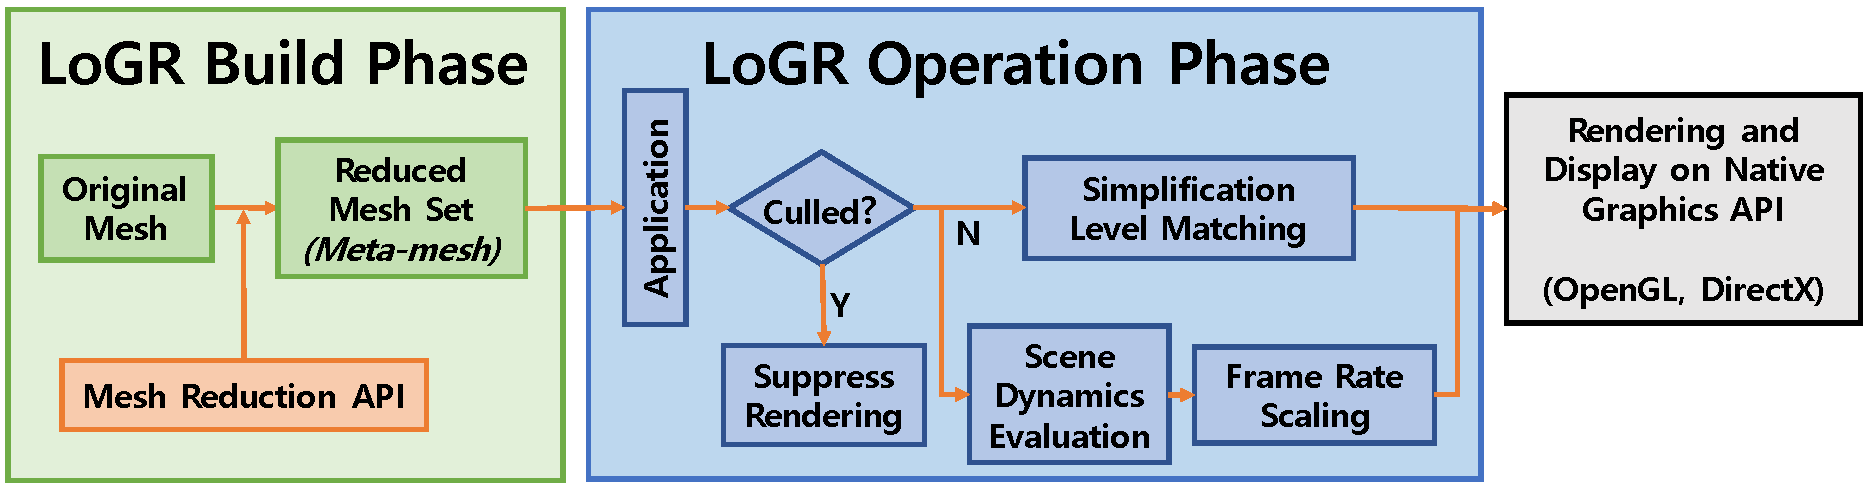
\includegraphics[width=1\linewidth]{scheme_cropped}
    \vspace{-2ex}
    \caption{{\myit} -- 
           the architecture and its functions.}
    \label{fig:lpglDiagram}
\end{figure}

With these goals in mind, we design {\myit}, a Low-power Graphics Library
for mobile AR headset applications.
%
In the software stack, {\myit} is positioned between the application and the 
system's native graphics library (e.g., OpenGL, DirectX)
(\fig\ref{fig:lpglDiagram}).
%
To the application, {\myit} provides OpenGL ES compatible front-end APIs.
%
For an application that uses these APIs, {\myit} intercepts the 
graphics-related calls to understand what the application targets to draw
(e.g., type/location of drawing, quantity of models).
%
In addition, {\myit} obtains user view points from the headset to gather
user perception physics (e.g. angle of sight, gaze).
%
Then, these information are combined to optimize the drawing process with respect 
to other system parameters, such as the frame rate and geometric complexity, so
that power usage is reduced while minimizing user perceived quality loss.
%
The following subsections provide details on the {\myit} design.


%%%%%%%%%%%%%%%%%%%%%%%%%%%%%%%%% 80 CHAR %%%%%%%%%%%%%%%%%%%%%%%%%%%%%%%%%%%%%%

\subsection{{\myit} Front-end APIs}

Front-end APIs of {\myit} are designed to be compatible with the OpenGL
ES 3.0 APIs~\cite{opengl}. 
%, while adding a few additional {\myit}-specific APIs.
%
This results in no changes to the application's code and allows {\myit} 
to easily intercept and capture the contents to be drawn on the display.
%
Through the APIs, {\myit} hooks to the graphics-related calls from the application
and passes appropriate information to its sub-modules for further processing, prior to sending commands to the system's native graphic library.
%
%Specifically, the current implementation of {\myit} offers calls for the
%graphics library's geometry-related functions.


%%%%%%%%%%%%%%%%%%%%%%%%%%%%% REWRoTE %%%%%%%%%%%%%%%%%%%%%%%%%%%

%A major design goal of {\myit} is to achieve complete application transparency, meaning that we target to enforce no changes to the application code itself to use the {\myit} capabilities. 

To achieve this transparency, we design our software so that all {\myit} functionalities are enabled through compiler configurations. The application developer simply makes changes to the compiler configurations to use {\myit}, and at compile time, the source code binary and necessary 3D objects are modified to support the added features of {\myit}. 
%
These, compile time configurations allow {\myit} to intercept all graphics-related calls prior to entering the native graphics stack. Specifically, through this process we (1) initialize {\myit}, (2) configure a command queue in which application API calls can be gathered before being pushed to the system graphics stack, and (3) load a mesh with different complexities to perform mesh simplification as we will detail in Section~\ref{sec:mesh}. 


%\fig\ref{fig:api} presents {\myit}-specific APIs and an example
%OpenGL compatible wrapper API ({\small\tt glVertexAttribPointer()}) supported by 
%{\myit}.
%
%Here, {\myit}-specific APIs are special purpose APIs used for operating {\myit}.
%{\small\tt lpglInit()} initializes internal data structures such as the command 
%queue for hooking to a graphics call. {\small\tt lpglInit()} must be called to 
%use the {\myit} functionalities. 
%
%The command queue, a core data structure, gathers the application's API calls 
%until the {\small\tt lpglCommit()} command is issued. {\small\tt lpglCommit()}
%then pushes the commands through the {\myit} procedures and passes the (modified)
%commands to the native graphics stack.
%
%While OpenGL compatible APIs mimic native graphics API calls, in reality, calls
%made from the application are put into the {\myit} command queue for modifications
%at {\myit} components once {\small\tt lpglCommit()} is issued.
%
%In addition, when objects are created at the application, loading commands are 
%called to place the objects' geometries to the graphics buffer for the draw calls 
%to execute. At this phase, we introduce a third {\myit} command, {\small\tt 
%lpglLoad()}. This call allows {\myit} to simplify a target object's complexity as 
%we will detail in Section~\ref{sec:mesh}. 
%%%%%%%%%%%%%%%%%%%%%%%%%%%%%%%%%%%%%%%%%%%%%%%%%%%%%%%%%%%%%%%%%


%\begin{figure}[t]
%    \centering
%    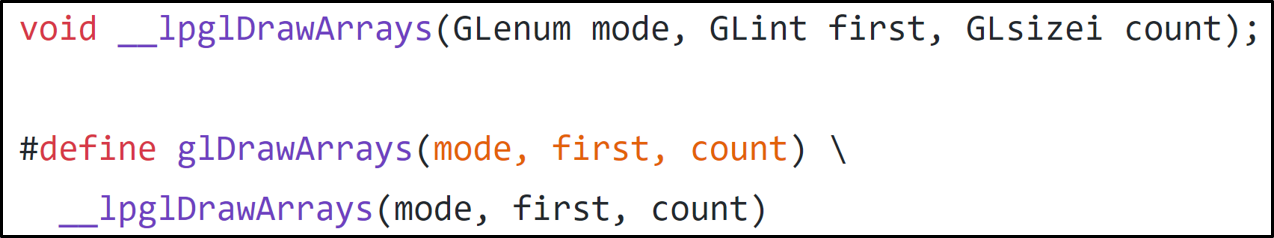
\includegraphics[width=1\linewidth]{lpglSourceCode}
%    \vspace{-2ex}
%    \caption{A Sample API example provided by {\myit}.
%            }
%    \label{fig:api}
%\end{figure}


% Internally, the native calls are preprocessed.
% In detail, we defined preprocessor function to mimic native OpenGL APIs.
% If application developer types OpenGL API for example 
% {\small\tt glDrawElementsInstanced()}, it is resolved to source code which 
% calls {\small\tt \_\_lpglDrawElementsInstanced()} by preprocessor.
% {\small\tt \_\_lpglDrawElementsInstanced()} function pushes their given 
% parameters to command queue.


OpenGL-compatible front-end APIs supported in {\myit} consists of two parts: 
APIs for initializing the drawing data, and APIs for the actual drawing.
%
The calls to the former contain information on what objects will be drawn,
%
including vertices and topology information. 
%(c.f., \fig\ref{fig:lpglDiagram}).
%
APIs for the actual object drawing are again divided into two categories:
%
transformation APIs apply geometric transformation
(e.g., scaling, rotation, translation) to the target object, and
%
draw calls send commands to draw objects to the GPU.
%by applying the transform functions to the vertex buffer configured in the
%initialization phase.


%%%%%%%%%%%%%%%%%%%%%%%%%%%%%%%%% 80 CHAR %%%%%%%%%%%%%%%%%%%%%%%%%%%%%%%%%%%%%%


\subsection{Mesh Simplification}
\label{sec:mesh}

As we saw in the preliminary studies, the number of triangles that consist 
a 3D object (i.e., object complexity) heavily impacts the power usage of a mobile AR application. 
%
However, when displaying multiple complex objects in a single scene, often the 
user's perception (e.g., direction of sight or gaze) is towards only a subset 
of the objects.
%
Therefore, it makes sense to simplify objects that are out of the user's 
focal angle to minimize the power used for processing these objects.

To do so, we start by identifying the number of triangles that an application 
intends to draw using the {\small\tt glBufferData()}
and {\small\tt glVertexAttribPointer()} calls in the OpenGL APIs,
which provides vertices and topology information. 


Next, to reduce the number of triangles that consist an object while 
maintaining visible quality, we apply \emph{mesh simplification}.
%
Mesh simplification %a well-studied topic in the graphics research community, 
is used in various graphics applications to minimize computation costs for less-focused
objects. Among various methods, we used Audodesk Maya's Mesh Reduction
API~\cite{polyReduce}. %The use of other methods are also easily applicable.


%%%%%%%%%%%%%%%%%%%%%%%%%%%%% REWRoTE %%%%%%%%%%%%%%%%%%%%%%%%%%%

However, mesh simplification can be computationally heavy when performed on
the mobile headset itself. Therefore, all potentially displayed objects in {\myit} are
simplified \textit{in compile time} to create two 
additional versions of simplified meshes. Here, one version is a ``less'' 
simplified version (level 1 simplification) and the other is heavily simplified 
(level 2). For simple memory loading, the geometries of the original, 
level 1 and level 2 simplification meshes are combined to form a ``meta-mesh'' of an object.
%All 3D objects will have two aliases of the original mesh, a level 1 mesh and a level 2 mesh.
We note that some applications dynamically load 3D objects in run-time. To reduce 
object complexity for those not simplified in compile time, {\myit} also includes
a light-weight mesh simplification scheme based on Quadric Error Metrics~\cite{Garland98}
to reduce mesh complexities in run-time.

In operation, the meta-mesh of the target object is loaded to the memory upon 
a display request. As soon as a decision is made on what version of the
object should be displayed, the meta-mesh is split, and only the geometry for the
target complexity mesh is passed to the GPU.% memory for further processing. 

%%%%%%%%%%%%%%%%%%%%%%%%%%%%%%%%%%%%%%%%%%%%%%%%%%%%%%%%%%%%%%%%%%%%

In determining when and what version of the object will be displayed, we utilize 
gaze tracking or head orientation information provided by the mobile headset. 
Based on geometric information on how far an object is away from the user's focal 
point, we divide the user's field of view (FOV) in three: core focal 
angle, near peripheral sight, and far peripheral sight. 
%
Assuming that the user's core focal angle is within $\epsilon^\circ$ from the
current focal point extracted from the gaze tracker or head orientation 
information, objects beyond this angle distance can be simplified. If the object 
is located 1-3$\times\epsilon^\circ$ away from the focal point, we present
the level 1 simplified mesh, and use level 2 for all objects farther away. 
%
%Based on findings from previous literature~\cite{Strasburger11}, we set $\epsilon^\circ$ to $10^\circ$ and validate this using experiments in Section~\ref{sec:inlab}.



%%%%%%%%%%%%%%%%%%%%%%%%%%%%%%%%% 80 CHAR %%%%%%%%%%%%%%%%%%%%%%%%%%%%%%%%%%%%%%

\subsection{Frame Rate Control}

Our preliminary results show that frame rate has significant impact on the 
system's power usage. However, its control should be done with care since 
low frame rates may drastically drop the user perceived quality.
%
%Thus, {\myit} aims to guarantee that users' application experience is only
%minimally (if at all) affected.
%
Frame rate control in {\myit} is designed based on the intuition that frame rate 
need not be constant across all visual contents~\cite{Lim18Adaptive}.
%
It should be kept high to maintain the original quality for contents that change
frequently (e.g., high level of scene dynamics), but can be lowered without loss
of user-perceived quality when contents are less dynamic.
%
To exploit this idea, {\myit} implements a {\it Scene Dynamics Scoring Module},
which determines and quantifies the scene dynamics of frame contents using the 
scene's geometric information.
%
Based on this score, the {\it Reactive Display Complexity Control Engine} 
(Section~\ref{sec:rdcc}) can determine an appropriate frame rate.
%for the display content.

For example, if we define a scene's dynamics as the difference 
between subsequent frames, image-based schemes that use 
full contextual information, such as the structural similarity (SSIM) or peak signal-to-noise ratio (PSNR) can be used~\cite{ssim,psnr}.
%
However, they require significant amount of computation,
% to calculate features from the entire screen, and 
thus unsuitable for resource limited mobile devices~\cite{ssim,Hwang:2017:RPO}.
%due to the computational and latency overheads.
%
% Work by Hwang et al. also realize such complexity issues and use grayscale 
% images to reduce the computation cost~\cite{\cite{Hwang:2017:RPO:3117811.3117841}}. 
%
% To compute frame similarity in real-time despite the complexity,
% image-based schemes may use lower-resolution images rather than full resolution, 
% but this would still make it difficult to adaptively control the granularity.
%
% Applications that show detailed level changes would require {\myit} to monitor
% changes in the image in finer granularity compared to rough image-changing 
% applications. For the applications that are less sensitive, performing 
% fine-grained computation can be a waste of resources.
%
Furthermore, with these schemes, it is difficult to compute scene dynamics until the frame is fully rendered for object rendering applications, .
%and the image is available in the display buffer. 
We find this and the memory copy from the GPU's frame buffer as computational waste.

Moreover, image-based metrics may not be sensitive enough for small portions
of changes in the scene. Take a case in which a small object such as a bullet
passes through the user's scene. The bullet will travel fast, but if we compute 
the SSIM/PSNR for the entire frame, the contextual changes will only be marginal. 
Such schemes can suggest that there is
only a small level of dynamics and decrease the frame rate accordingly. In 
applications where drawing is done on an object-basis, we need a scheme 
more centered towards the objects themselves, rather than the entire frame image. 

%are not sensitive to the small portion of changes of whole scene.
%In an example of a scene which a man is shooting gun,
%even if the bullet would be fast enough but it would be evaluated as a little changes and set lower framerate. However from user's point of view, the bullet will be blown with stuck, which can be expected to have a negative impact on the user experience.


Such observations led us to propose and design a \emph{Distance-based frame 
dynamics scoring module}, an \emph{object geometry-based} light-weight approach 
for determining scene dynamics.
%
In our approach, the scene dynamics is defined as the maximum distance change of 
objects within two consecutive frames computed over all objects in the scene. Note
that this distance is defined 
%in the 2D coordinate space 
on the user's view point perspective.
%, not in the global 3D space. 
Therefore, even when the object is stationary and the user's view point changes 
(e.g., motions with the mobile AR device), the the dynamics can be captured.
%
To minimize computation costs, instead of using the original detailed coordinates 
of the 3D object, we set a ``bounding-box'', which is a box that best fits all the 
coordinates of the original object, and only compute the distance based on the 
box's center point. 
%
Such an approach allows {\myit} to compute the dynamics level of the scene 
before the scene is rendered, to suppress any unnecessary rendering and memory 
copy operations.

% However geometry-based method can not detect color and texture differences for non-moving objects. \jw{How about move the story about color and texture to discuss section?}
%

% \jk{add geometry distance-based method...}

% \jk{note the fact that this approach can capture things that PSNR/SSIM cannot capture. We are not focusing on the entire frame but if one object makes a fast motion, even if the object is small, we see the need to increase the frame rate.}

% \jk{limitation of geometry-based schemes is that we cannot capture changes in color/texture for non-moving objects}

%%%%%%%%%%%%%%%%%%%%%%%%%%%%%%%%% 80 CHAR %%%%%%%%%%%%%%%%%%%%%%%%%%%%%%%%%%%%%%

\subsection{Culling}

In addition to frame rate, the number of draw calls also impact the power 
consumption of a mobile AR headset.
%
Issuing draw calls are essential for drawing objects to the display, but 
executing draw calls for objects that cannot be physically seen 
(e.g., object out of current scene boundaries) would be a waste.
%
The most widely used graphics pipelines already exploit ``view frustum culling'' 
to account for such cases~\cite{}. The process of culling determines whether or not there 
is a chance for the target object to be observed 
%in the current scene, 
and suppresses the drawing if not.
%
%Specifically, in view frustum culling, once triangles complete vertex shading,
%the culling module checks if the object is outside of the ``view frustum'' 
%constructed using the gaze direction, FOV, and visible range.
%
%If an object is inside the view frustum, it is visible. Otherwise,
%culling suppresses the remaining graphics pipeline tasks, allowing the 
%system to conserve resources. 


%While culling itself is very important in saving energy and is already widely
While culling itself is already widely used, we've identified a point in which 
the main philosophy of ``not processing unseen objects'' can be further exploited 
to reduce power consumption even more.
%
In currently used view frustum culling, when a user is observing an object in the $x^\circ$ field, objects in the $x+180^\circ$ range 
will still be processed and pay the computation cost up to the point where the object geometries are known to the graphics library after being fully transformed to the 3D space.
%
%vertex shader
%before it is discarded. \jk{change this part a bit...}
%
%Surprisingly, this occurs for all well-known graphics libraries 
%since the geometry of the object is not known to the library until the 
%object is transformed on the 3D space.
%
However, objects beyond peripheral vision can not be seen, and we propose to 
eliminate \textit{all} the waste in the culling process.


Again, we exploit the user perception data, geometry information 
of all objects, and apply the bounding box-based approach.
%
By doing so, instead of transforming all vertices to the 3D space, we can selectively transform just the eight corner points that consist the bounding box. 
%
We infer the user's position in the 360$^\circ$ space, and use it to 
compute the angular distance $\tau^\circ$ between the user's view point direction 
vector and the vector of the object bounding box's center position.
%
Then, given a typical user's maximum FOV, if $\tau^\circ$ is not included in the 
FOV, we determine that there is no chance for the target object to be seen in the 
current scene.
%
Using this simple method, {\myit} improves view frustum culling and suppresses the
entire graphics pipeline process.

%\jk{I don't see how this is different from baseline}

%%%%%%%%%%%%%%%%%%%%%%%%%%%%%%%%% 80 CHAR %%%%%%%%%%%%%%%%%%%%%%%%%%%%%%%%%%%%%%

\subsection{Reactive Display Complexity Control}
\label{sec:rdcc}

%\jk{Change so that different levels are reflected in the text.}

%So far, we have discussed how {\myit} captures information from the application,
%how the meshes can be simplified and displayed based on the user's sight,
%how we quantify frame dynamics to control the frame rate,
%and how the culling process can be optimized to minimize the number of draw calls.
%
The mesh simplification, scene dynamics scoring, and culling techniques
discussed until now are designed based on the idea that we can utilize the
relationship between the user's view point (from the gaze tracker) and the 
object's geometry.
%
To effectively combine all {\myit} features, 
we design the Reactive Display Complexity Control (RDCC) engine.
%
The RDCC engine offers a framework that exploits the three core features of
{\myit} with minimal computational overhead, and provides a fine-grained 
display control environment. 
%
Through RDCC, {\myit} reactively controls graphics-related parameters 
based on the user's perception of the scene. 

A key idea of the RDCC engine in {\myit} is to focus the computation on only the 
bounding-box surrounding the geometry rather than the full geometric information.
%
Take the culling process for example, which is interested in identifying 
whether the target object is within the user perceived scene or not.
%
Given that the bounding box provides the minimum and maximum points of the object,
if we simply identify that the bounding box is outside the user's sight, we can
easily remove this object from the graphics pipeline.
%
Similarly for frame rate control and mesh simplification, the RDCC engine makes
its decisions based on features (e.g., scene dynamics or object position) extracted from the bounding box. 

Overall, RDCC operates as follows. For each object draw call, the culling process first takes place after identifying the object's bounding box. Then a mesh of 
a proper detail (e.g., original object or simplified mesh) is presented 
after determining that the object is currently within the core focal angle or near 
peripheral angle. Finally, the target frame rate is set 
based on the objects' dynamics in the scene to project them through native graphics 
library's drawing APIs.


%As for the frame rate, the RDCC engine determines when the next frame will be 
%displayed based on the current value of the frame dynamics score. 
%
%High level of dynamics will result in high frame rate, and a low dynamics score
%will lead to a lower frame rate.
%
%This decision is based on a set of parameters which determine at what 
%dynamics level the frame rate will ``shift" to a different level.


%Finally for mesh simplification, the RDCC engine takes the role of confirming
%if an object's bounding box is within $\epsilon^\circ$ of the center of focus 
%or not with respect to the head direction
%extracted from the gyroscope sensor.
%
%Since, the bounding box of an object is a common feature that all three 
%components in {\myit} use, the RDCC engine extracts this 
%information prior to processing the object in different components. 


%%%%%%%%%%%%%%%%%%%%%%%%%%%%%%%%% 80 CHAR %%%%%%%%%%%%%%%%%%%%%%%%%%%%%%%%%%%%%%

%\subsection{{\myit} Parameter Selection}
%\label{sec:parameters}


%Given the design discussed until now, 
%it is important that {\myit} offers proper controllable parameters so that 
%its functionalities can be effectively exposed.
%
%Current implementation of {\myit} offers three major parameters.
%
%First is $d_B$, the binary tree depth parameter for controlling the mesh 
%simplification level.
%With a small $d_B$, the 3D objects are represented with only a small number of
%voxels, which reduces the quality of the object, but maximizes energy efficiency.
%A large $d_B$ on the other hand, will provide a fine-grained and detailed 
%object projection, but limits the energy reduction.
%
%In this phase, $min_{vx}$ can also be configured to set the level of filtering
%adjacently created triangles. While this value can be variable, current 
%implementation of {\myit} fixes this value to 30 based on a number of object
%quality measurements.


%The second controllable parameter in {\myit} is $d_Q$, the depth metric for
%determining frame dynamics. A high $d_Q$ will provide a very detailed 
%summary of the changes occurring on two consecutive frames, while a small 
%$d_Q$ will provide information on easily noticeable, larger differences.
%
%The resulting frame dynamics score $DS_n$, is compared with a threshold $DT_n$
%that specifies when the RDCC engine should determine to transition to a 
%new display frame rate.
%
%This process should define a set of thresholds for shifting the frame rate
%from $FR_1$ to $FR_2$, for example.
%When configuring the target frame rate $FR_n$ in multiple steps, thresholds 
%$DT_n (n=1,2,3,...)$ should be defined for each frame rate transition state. 


%Note that the currently {\myit} allows the application to 
%choose these parameters, and does not offer preset values.
%Configuring preset values or autonomously adapting these parameters on a 
%per-user (or-per application) basis requires deeper user studies and we 
%leave this as part of future work. 

%%%%%%%%%%%%%%%%%%%%%%%%%%%%%%%%% 80 CHAR %%%%%%%%%%%%%%%%%%%%%%%%%%%%%%%%%%%%%%

